\documentclass[12pt]{article} % размер шрифта

\usepackage{tikz} % картинки в tikz
\usepackage{microtype} % свешивание пунктуации

\usepackage{array} % для столбцов фиксированной ширины

\usepackage{url} % для вставки ссылок \url{...}

\usepackage{indentfirst} % отступ в первом параграфе

\usepackage{sectsty} % для центрирования названий частей
\allsectionsfont{\centering} % приказываем центрировать все sections

\usepackage{amsthm} % теоремы и доказательства

\theoremstyle{definition} % прямой шрифт в условии теорем
\newtheorem{theorem}{Теорема}[section]


\usepackage{amsmath, amssymb} % куча стандартных математических плюшек

\usepackage[top=2cm, left=1.5cm, right=1.5cm, bottom=2cm]{geometry} % размер текста на странице

\usepackage{lastpage} % чтобы узнать номер последней страницы

\usepackage{enumitem} % дополнительные плюшки для списков
%  например \begin{enumerate}[resume] позволяет продолжить нумерацию в новом списке
\usepackage{caption} % подписи к картинкам без плавающего окружения figure

\usepackage{hyperref} % гиперссылки

\usepackage{verbatim} % побуквенный вывод

\usepackage{fancyhdr} % весёлые колонтитулы
\pagestyle{fancy}
\lhead{Эконометрика, финтех}
\chead{}
\rhead{2018-11-10, встреча 6}
\lfoot{}
\cfoot{}
\rfoot{\thepage/\pageref{LastPage}}
\renewcommand{\headrulewidth}{0.4pt}
\renewcommand{\footrulewidth}{0.4pt}



\usepackage{todonotes} % для вставки в документ заметок о том, что осталось сделать
% \todo{Здесь надо коэффициенты исправить}
% \missingfigure{Здесь будет картина Последний день Помпеи}
% команда \listoftodos — печатает все поставленные \todo'шки

\usepackage{booktabs} % красивые таблицы
% заповеди из документации:
% 1. Не используйте вертикальные линии
% 2. Не используйте двойные линии
% 3. Единицы измерения помещайте в шапку таблицы
% 4. Не сокращайте .1 вместо 0.1
% 5. Повторяющееся значение повторяйте, а не говорите "то же"

\usepackage{fontspec} % поддержка разных шрифтов
\usepackage{polyglossia} % поддержка разных языков

\setmainlanguage{russian}
\setotherlanguages{english}

\setmainfont{Linux Libertine O} % выбираем шрифт
% если Linux Libertine не установлен, то
% можно также попробовать Helvetica, Arial, Cambria и т.Д.

% чтобы использовать шрифт \Linux Libertine на личном компе,
% его надо предварительно скачать по ссылке
% http://www.\Linuxlibertine.org/index.php?id=91&L=1

% на сервисах типа sharelatex.com этот шрифт есть :)

\newfontfamily{\cyrillicfonttt}{Linux Libertine O}
% пояснение зачем нужно шаманство с \newfontfamily
% http://tex.stackexchange.com/questions/91507/

\AddEnumerateCounter{\asbuk}{\russian@alph}{щ} % для списков с русскими буквами
\setlist[enumerate, 2]{label=\asbuk*),ref=\asbuk*} % списки уровня 2 будут буквами а) б) ...

%% эконометрические и вероятностные сокращения
\DeclareMathOperator{\Cov}{Cov}
\DeclareMathOperator{\sCov}{sCov}
\DeclareMathOperator{\sVar}{sVar}
\DeclareMathOperator{\sCorr}{sCorr}
\DeclareMathOperator{\Corr}{Corr}
\DeclareMathOperator{\Var}{Var}
\DeclareMathOperator{\E}{E}
\DeclareMathOperator{\tr}{trace}
\DeclareMathOperator{\trace}{trace}
\DeclareMathOperator{\Lin}{Lin}
\DeclareMathOperator{\Linp}{Lin^{\perp}}
\DeclareMathOperator{\col}{col}
\DeclareMathOperator{\colp}{col^{\perp}}

\def \hb{\hat{\beta}}
\def \hs{\hat{\sigma}}
\def \htheta{\hat{\theta}}
\def \s{\sigma}
\def \hy{\hat{y}}
\def \hY{\hat{Y}}
\def \hu{\hat{u}}
\def \v1{\vec{1}}
\def \e{\varepsilon}
\def \he{\hat{\e}}
\def \z{z}
\def \hVar{\widehat{\Var}}
\def \hCorr{\widehat{\Corr}}
\def \hCov{\widehat{\Cov}}
\def \cN{\mathcal{N}}
\def \RR{\mathbb{R}}

\makeatletter
\def\MT@warn@unknown{}
\makeatother




\begin{document}

Конспектировала: Мария Щеголева.

\section{Нормальное распределение}


Путь через теорему Хершела-Максвелла: \textit{Если распределение случайного вектора с независимыми компонентами инвариантно к повороту, то компоненты вектора распределены нормально }.

\begin{center}
    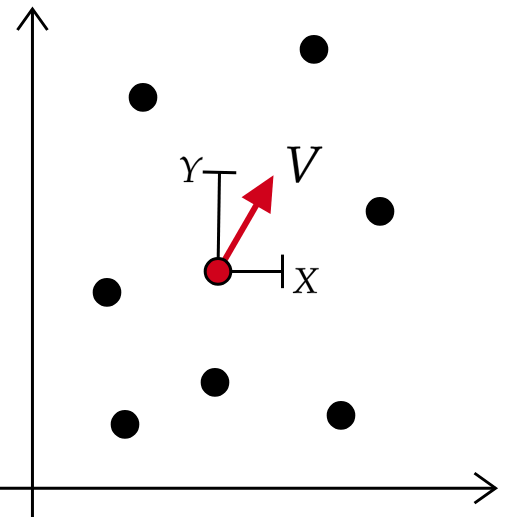
\includegraphics[width=5cm]{images/pic01_06.png}
\end{center}

\newtheorem{axiom}{Аксиома}
\begin{axiom}\label{ax1}
    Закон распределения вектора скорости $ V = \begin{pmatrix} X \\ Y \end{pmatrix}$ не зависит от направления, а только от длины: $f(x,y) = h(x^2+y^2)$
\end{axiom}

\begin{axiom}\label{ax2}
    Компоненты скорости $X$ и $Y$ независимы: $ f(x,y) = g_X(x)\cdot{g_Y(y)} $
\end{axiom}

\begin{axiom}\label{ax3}
    Нормировка: $\Var(X) = 1$
\end{axiom}

\textit{Cвойства}: \par
Пусть вектор $V'$ получен поворотом вектора $V$. По Аксиоме~(\ref{ax1}) операция поворота не меняет распределение вектора $V \hspace{0.2cm} \Rightarrow \hspace{0.2cm} V' \sim V$:
\bigskip
%\subitem{
\[
\begin{pmatrix}
  X \\
  Y
\end{pmatrix} \xrightarrow{\circlearrowleft \space 180^{\circ}}
\begin{pmatrix}
  -X \\
  -Y
  \end{pmatrix} \hspace{0.3cm}
  \Rightarrow \hspace{0.3cm} X \sim -X \hspace{0.3cm}
  \Rightarrow \hspace{0.3cm} \E(X)=0
\]
% }
\medskip
%\subitem{
\[
\begin{pmatrix}
  X \\
  Y
\end{pmatrix} \xrightarrow{\circlearrowleft \space 90^{\circ}}
\begin{pmatrix}
  Y \\
  -X
\end{pmatrix} \hspace{0.3cm} \Rightarrow \hspace{0.3cm} X \sim Y, \; Y \sim -X \hspace{0.3cm}
\Rightarrow \hspace{0.3cm} \E(X)=\E(Y)=0; \Var(Y)=\Var(X)=1
\]
%}  \\

\newtheorem*{define}{Определение}
\begin{define}
Вектор $ V = \begin{pmatrix} X \\ Y \end{pmatrix}$ имеет \emph{стандартное нормальное распределение}, если верны Аксиомы~(\ref{ax1})--(3).
\end{define}

\begin{proof} \hspace{1cm}
    \begin{itemize}
        \item[ ] По Аксиоме~(\ref{ax1}): $f(x,y) = h(x^2+y^2)$. По Аксиоме~(\ref{ax2}) компоненты вектора $V$ независимы, а из полученных свойств имеют одинаковое распределение ($X \sim Y \hspace{0.1cm} \Rightarrow \hspace{0.1cm} g_X=g_Y$), следовательно функция плотности совместного распределения может быть представлена как произведение функций плотности маргинальных:
    \end{itemize}
    \centering $f(x,y)=g(x^2)\cdot g(y^2)$ \pagebreak
    \[
        h(x^2+y^2) = g(x^2) \cdot g(y^2)
    \]
    \[
        \begin{cases}
            h'(x^2+y^2) = g'(x^2) \cdot g(y^2)\\
            h(x^2+y^2) = g(x^2) \cdot g(y^2)
        \end{cases}
        \xrightarrow{x=0} \hspace{0.5cm}
        \begin{cases}
            h'(y^2) = g'(0) \cdot g(y^2)\\
            h(y^2) = g(0) \cdot g(y^2)
        \end{cases}
    \]
    \[
        h'(t) = \frac{g'(0)}{g(0)}h(t)
        \hspace{0.5cm} \Rightarrow \hspace{0.5cm}
        h'(t) = k \cdot h(t)
        \hspace{0.5cm} \Rightarrow \hspace{0.5cm}
        h(t)=c \cdot e^{kt}
    \]
    \[
        f(x,y) = c \cdot e^{k(x^2+y^2)} = \sqrt{c} \cdot e^{kx^2} \cdot \sqrt{c} \cdot e^{ky^2} = g(x) \cdot g(y)
    \]

    \begin{itemize}[label={$\bullet$}]
        \item $k - ?$
            \[
            \E(X^2) = \int\limits_{-\infty}^{+\infty} x^2 \sqrt{c} \cdot e^{kx^2} dx = 1
            \]
            Интегрируем по частям:
            \[
             \int\limits_{-\infty}^{+\infty} x \sqrt{c} \cdot x \cdot e^{kx^2} dx = x \cdot \sqrt{c} \cdot e^{kx^2} \cdot \frac{k}{2} \bigg\vert_{-\infty}^{+\infty} - \int\limits_{-\infty}^{+\infty} \sqrt{c} \cdot e^{kx^2} \cdot \frac{1}{2k} dx = - \frac{1}{2k} \int\limits_{-\infty}^{+\infty} \sqrt{c} \cdot e^{kx^2} = - \frac{1}{2k}
            \]
            \[
            - \frac{1}{2k} = 1  \hspace{0.5cm} \Rightarrow \hspace{0.5cm}
            k = - \frac{1}{2}
            \]

        \item $c - ?$
            \[
                f(x,y) = c \cdot e^{-\frac{1}{2}(x^2+y^2)}
            \]
            Объем под функцией плотности:
            \[
                I = \int\limits_{-\infty}^{+\infty}\int\limits_{-\infty}^{+\infty} c \cdot e^{-\frac{1}{2}(x^2+y^2)}dxdy = 1
            \]

            \underline{Способ 1:} Перейти к полярным координатам \\
            \[
            dx \wedge dy = d(r\cos{\phi}) \wedge d(r\sin{\phi}) = rd\phi \wedge d\phi
            \]
            \par \underline{Способ 2:}(почти устно) Найти объем \par
            \smallskip
            \textbf{Принцип Кавальери:}
            \begin{center}
               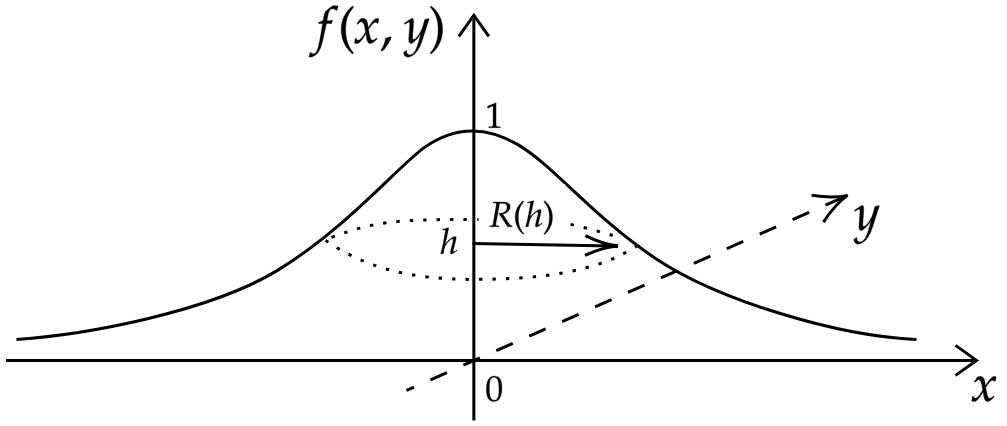
\includegraphics[width=9cm]{images/pic02_06.png}
            \end{center}
            \[
            I = c \int\limits_{0}^{1}\pi R^2(h) dh =
            \Bigg[h = e^{-\frac{1}{2}R^2(h)} \hspace{0.2cm} \Rightarrow \hspace{0.2cm} R^2(h) = -2\log(h)\Bigg] = c \int\limits_{0}^{1} -2\pi \log(h) dh
            \]
            \newpage
            Замена переменной и пределов интегрирования: $I = -2\pi \cdot c \int\limits_{-\infty}^{0}e^{x}dx$
            \begin{center}
               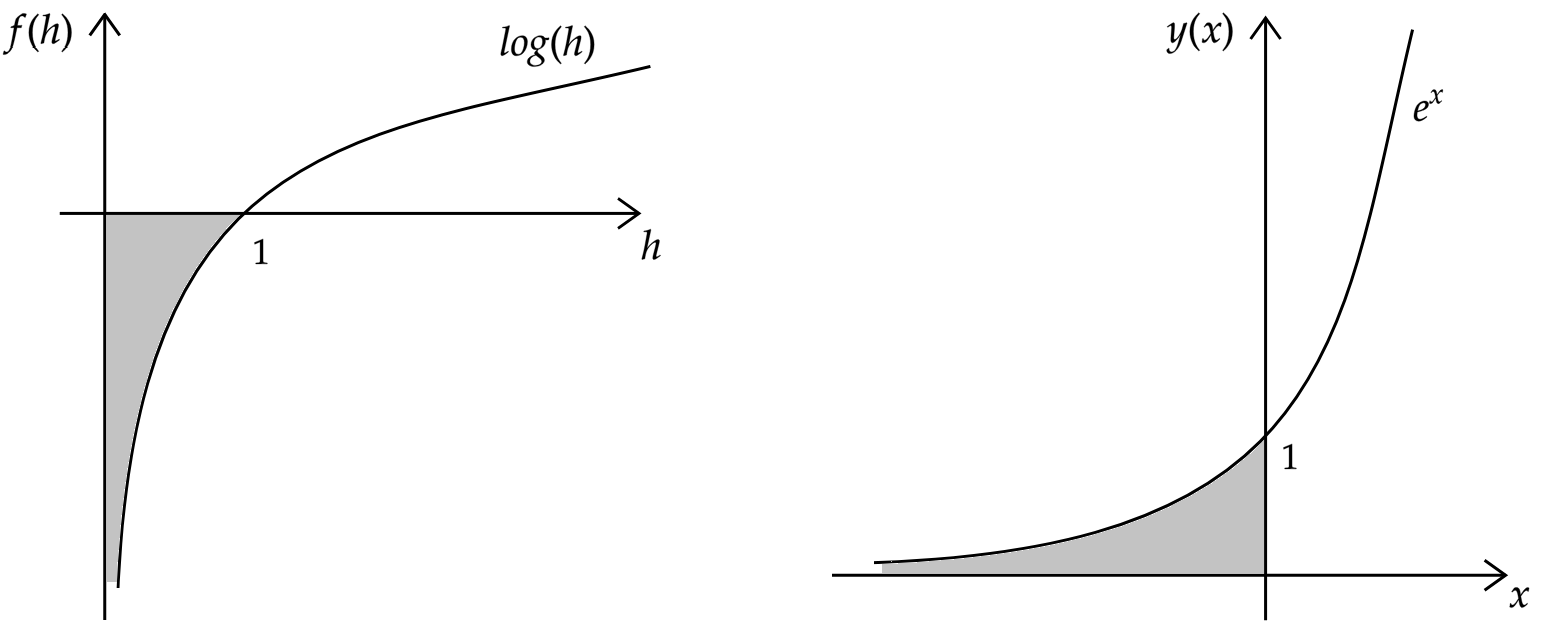
\includegraphics[width=11cm]{images/pic03_06.png}
            \end{center}

            \textbf{Геометрическое свойство экспоненты:}\par
            \begin{center}
               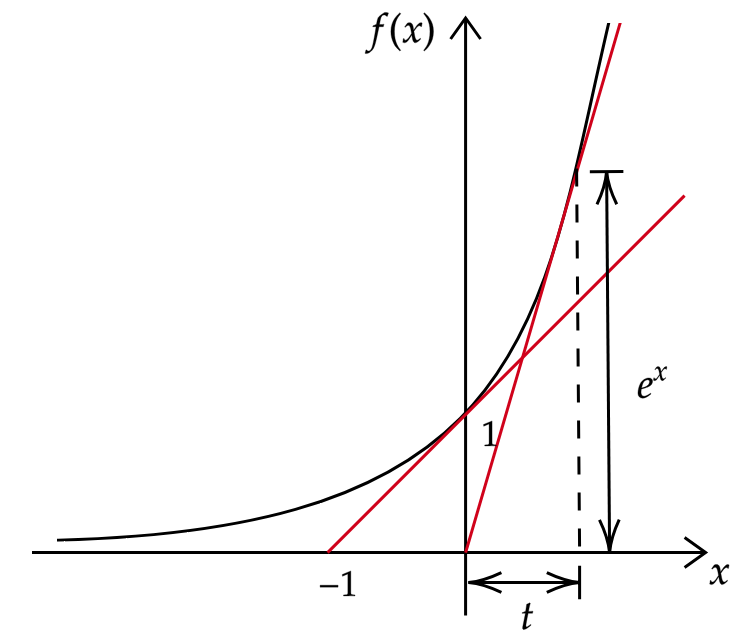
\includegraphics[width=6cm]{images/pic04_06.png}
            \end{center}
            \[
            (e^x)' = e^x \hspace{0.2cm} \Rightarrow \hspace{0.2cm} \tg \alpha = e^x \hspace{0.2cm} \Rightarrow  \hspace{0.2cm} \frac{e^x}{t} = e^x \hspace{0.2cm} \Rightarrow \hspace{0.2cm} t = 1
            \] \par

            \textbf{Принцип Мамикона}: \par
            Площадь $S$, закрашиваемая касательными при движении вдоль кривой, равна площади, закрашиваемой касательными, если только поворачивать их, но не перемещать вдоль кривой, независимо от формы исходной кривой.\par
            \begin{center}
               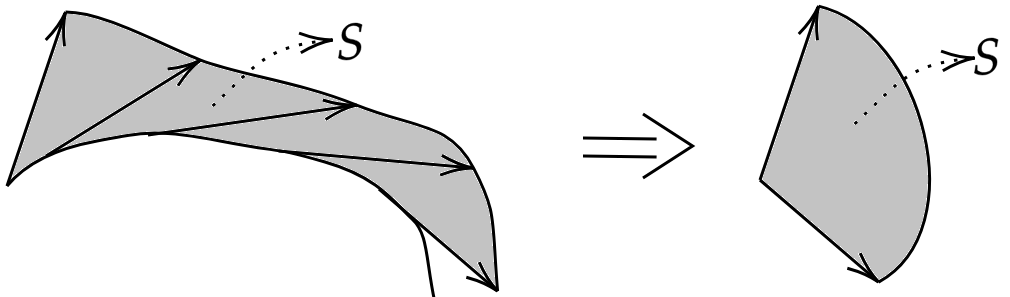
\includegraphics[width=7cm]{images/pic05_06.png}
            \end{center}
            Площадь фигуры, которую закрашивают касательные при движении по кривой $e^x$ от $-\infty$ до $0$, по принципу Мамикона равна $\frac{1}{2}$. Тогда $\int\limits_{-\infty}^{0}e^{x}dx$ равен сумме площади серой фигуры, закрашенной касательными, и площади треугольника ($S_{\Delta}=\frac{1}{2}\cdot 1 \cdot 1$):
            \begin{center}
               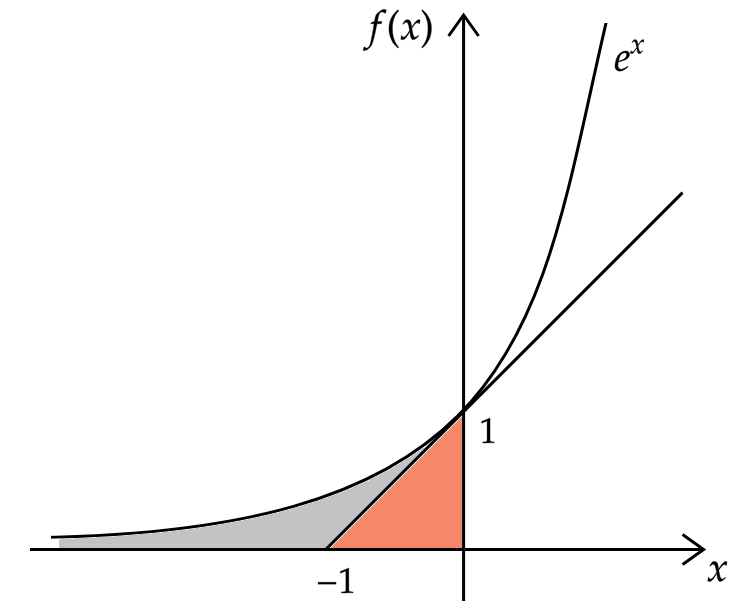
\includegraphics[width=6cm]{images/pic06_06.png}
            \end{center}
            \[
            I = -2\pi \cdot c \int\limits_{-\infty}^{0}e^{x}dx = -2\pi \cdot c \cdot \Big(\frac{1}{2} + \frac{1}{2}\Big) = 1 \hspace{0.2cm} \Rightarrow \hspace{0.2cm} c = -\frac{1}{2\pi} \] \par
            \[
             f(x,y) = -\frac{1}{2\pi} \cdot e^{-\frac{1}{2}(x^2+y^2)} \hspace{0.2cm} \Rightarrow \hspace{0.2cm} X \sim \cN(0, 1), Y \sim \cN(0, 1)
            \]
    \end{itemize}

    \emph{Замечание:} Без Аксиомы (\ref{ax3}) $X$, $Y$ имеют нормальное распределение $\sim \cN(0, \sigma^2)$.
\end{proof}


\section{$\chi^2$-распределение}

\begin{define}\label{d1}
    Если вектор $y = (y_1, \hdots, y_n)^T$ имеет стандартное нормальное распределение ( $y_i \sim \cN(0, 1)$, $y_i$ — независимы), $V$ — $k$-мерное подпространство, $\hy$ — проекция $y$ на $V$ и $q = \lVert \hy \rVert^2$ — квадрат длины проекции, то $q$ имеет $\chi^2$-распределение с $k$ степенями свободы.
\end{define}

\newtheorem*{classic_def}{Классическое определение}
\begin{classic_def}\label{cd1}
    Случайная величина $q$ имеет $\chi_k^2$-распределение, если $q$ представима в виде $q = z_1^2 + z_2^2 + \hdots + z_k^2$, где $z_i \sim \cN(0, 1)$ и независимы.
\end{classic_def}
\smallskip
\emph{Эквивалентность:} если $n=k$ и $V$ — все пространство, тогда $y = \hy$ и $q = \lVert \hy \rVert ^2 = y_1^2 + y_2^2 + \hdots + y_k^2$ \par
\smallskip
\newtheorem*{exerc}{Упражнение}
\begin{exerc}
    Вектор $( y_1, y_2, y_3 ) ^T$ имеет стандартное нормальное распределение; $V=\{y_1 + y_2 = y_3\}$ — двумерное подпространство.\par
    \medskip
    Найдите вектор $\hy$, проекцию вектора $y$ на пространство $V$,
    и квадрат длины этой проекции.
    \[
    \hat y = Hy; \hspace{1cm} H = (X^TX)^{-1}X^Ty
    \]
    \par Базисные векторы подпространства $V$: \hspace{0.5cm}
    $X = \begin{pmatrix} 1 & 0 \\ 0 & 1 \\ 1 & 1 \end{pmatrix}$ \par
    \[
    X^TX = \begin{pmatrix} 2 & 1 \\ 1 & 2 \end{pmatrix}; \hspace{0.5cm}     (X^TX)^{-1} = \frac{1}{3} \begin{pmatrix} 2 & -1 \\ -1 & 2 \end{pmatrix}
    \]
    \[
    H = \begin{pmatrix} 1 & 0 \\ 0 & 1 \\ 1 & 1 \end{pmatrix} \cdot \frac{1}{3} \begin{pmatrix} 2 & -1 \\ -1 & 2 \end{pmatrix} \cdot \begin{pmatrix} 1 & 0 & 1 \\ 0 & 1 & 1 \end{pmatrix} = \frac{1}{3} \begin{pmatrix} 2 & -1 & 1 \\ -1 & 2 & 1 \\ 1 & 1 & 2\end{pmatrix}
    \]
    \[
    \hat y = \frac{1}{3} \begin{pmatrix} 2 & -1 & 1 \\ -1 & 2 & 1 \\ 1 & 1 & 2\end{pmatrix} \cdot \begin{pmatrix} y_1 \\ y_2 \\y_3 \end{pmatrix} = \begin{pmatrix} \frac{1}{3} (2y_1 - y_2 + y_3) \\ \frac{1}{3} (-y_1 + 2y_2 + y_3) \\ \frac{1}{3} (y_1 + y_2 + 2y_3) \end{pmatrix}
    \]
    \[
    q = \Big( \frac{2y_1 - y_2 + y_3}{3}\Big)^2 +\Big( \frac{-y_1 + 2y_2 + y_3}{3}\Big)^2 + \Big( \frac{y_1 + y_2 + 2y_3}{3}\Big)^2
    \]
    \par По классическому определению:  $q \sim \chi_2^2$
\end{exerc}
\smallskip
\newtheorem*{theo_n}{Теорема}
\begin{theo_n}
    Если $y=X\beta+u$; $u_i \sim \cN(0, \sigma^2)$ и независимы, то $\frac{RSS}{\sigma^2} \sim \chi_{n-k}^2$
\end{theo_n}

\begin{proof} \hspace{1cm} \par
    \smallskip
    $\hy$ — проекция $y$ на $\col(X)$ — пространство столбцов $X$. $\dim(\col(X)) = k$. \par
    Пространство $V = \colp(X)$ — ортогональное дополнение к $\col(X)$. $\dim(V) = n - k$. \par
    Матрица $(I-H)X\beta$ — проекция $X\beta$ на $V$. Заметим, что $X\beta \perp V$, следовательно $(I-H)X\beta = 0$. \par
    $\hu$ — проекция $u$ на $V$, поэтому $\hu = (I-H)y = (I-H)(X\beta + u) = (I-H)u$. \par
    По условию: $u_i \sim \cN(0, \sigma^2) \hspace{0.5cm} \Rightarrow \hspace{0.5cm} \cfrac{u_i}{\sigma} \sim \cN(0, 1)$. \par
    \smallskip
    Тогда по определению: $\cfrac{RSS}{\sigma^2} = \cfrac{\lVert (I-H)u \rVert^2}{\sigma^2} = \Big\lVert (I-H)\cfrac{u}{\sigma} \Big\rVert^2 \sim \chi_{n-k}^2$, где $\Big\lVert (I-H)\cfrac{u}{\sigma} \Big\rVert^2$ — длина проекции $\Big\{ \cfrac{u_i}{\sigma} \sim \cN(0,1)\Big\}_n$ на подпространство $V$.
\end{proof}

\begin{exerc}
    Вектор $y = u$. Вектор $u$ имеет нормальное распределение: $ u_i \sim \cN(0,\sigma^2)$ и независимы. Оценивается модель $\hy = X\hb$ по МНК.

    \begin{itemize}
        \item $TSS = \sum (y_i - \bar y)^2$
            \begin{center}
               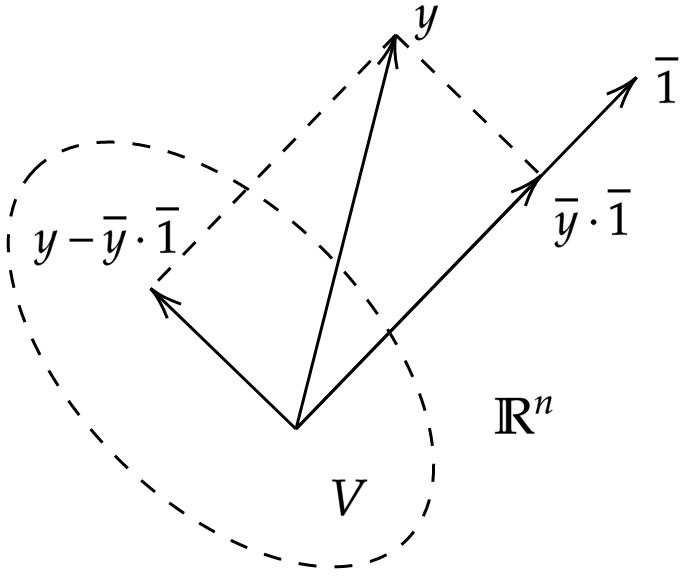
\includegraphics[width=6cm]{images/pic07_06.png}
            \end{center}
            $TSS = \lVert y - \bar y \cdot \bar 1 \rVert^2$ — длина проекции $y$ на подпространство $V = \Linp \bar 1 $ — ортогональное дополнение к $\bar 1$ из $\col(X)$ в пространстве $\RR^n$, поэтому $\dim V =n-1$
            \[
            \frac{TSS}{\sigma^2} \sim \chi_{n-1}^2
            \]
        \newpage
        \item $ESS = \sum (\hat {y_i} - \bar y)^2$
            \begin{center}
               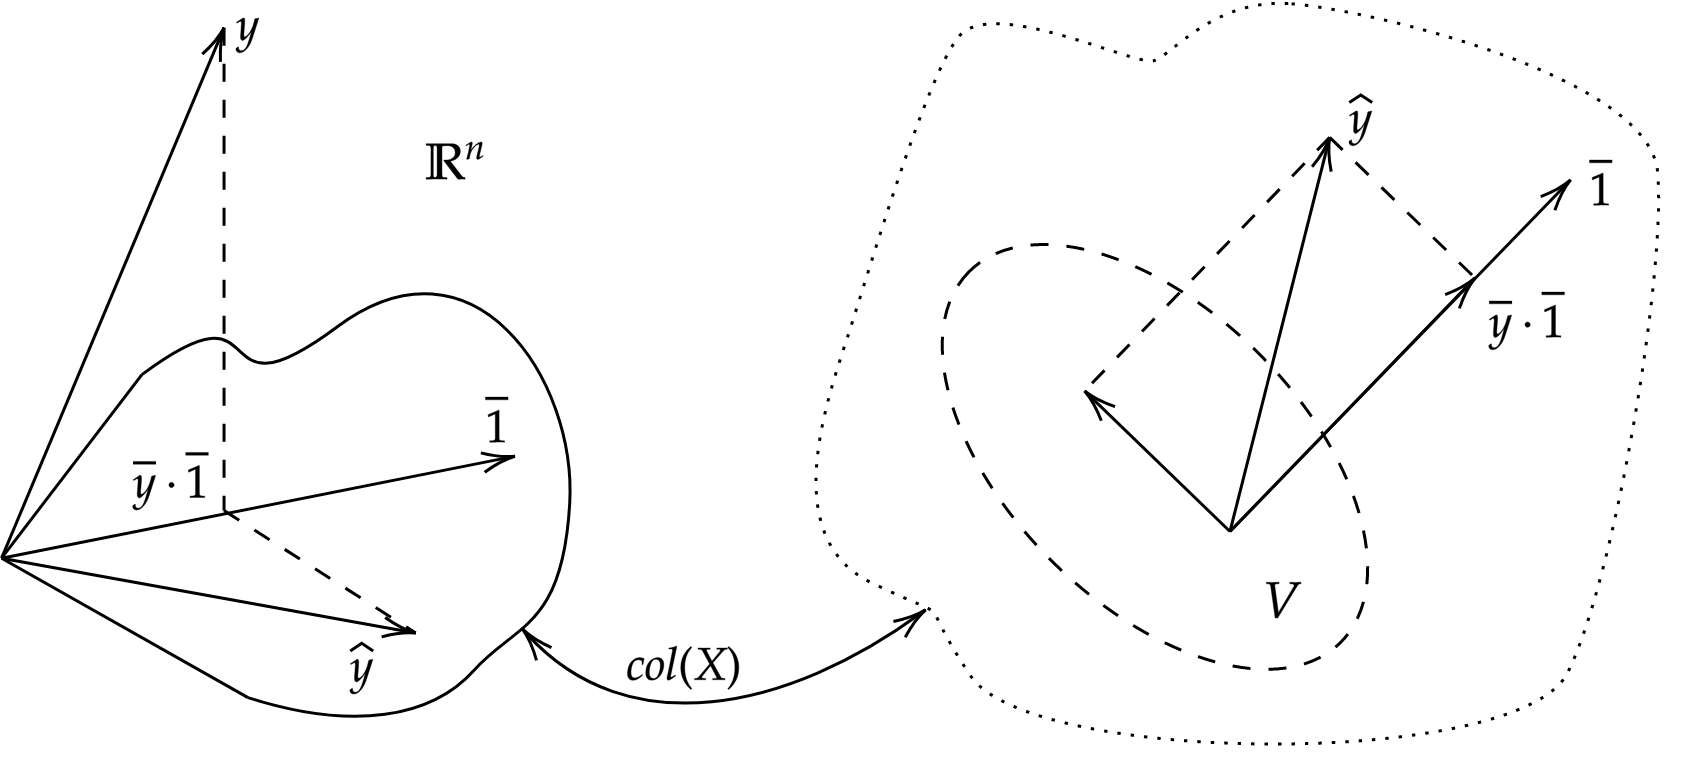
\includegraphics[width=12cm]{images/pic08_06.png}
            \end{center}
            $ESS = \lVert \hat y - \bar y \cdot \bar 1 \rVert^2$ — длина проекции $y$ на подпространство $V = \Linp \bar 1 \cap \col(X)$ — ту часть $\col X $, которая лежит в ортогональном дополнении к $\bar 1$, поэтому $\dim V =k-1$
            \[
            \frac{ESS}{\sigma^2} \sim \chi_{k-1}^2
            \]
    \end{itemize}
\end{exerc}
\smallskip
\newtheorem*{statem}{Удобное следствие}
\begin{statem}
    Аксиома (\ref{ax1}) $+$ Аксиома (\ref{ax2}) $=$ длины проекций на ортогональные подпространства независимы.
\end{statem}
\begin{proof} \hspace{1cm} \par
    \smallskip
    $y = (y_1, \hdots, y_n)^T$ $y_i \sim \cN(0, \sigma^2)$ и независимые.\par
    $W, V$ — подпространства в $\RR^n$; $V \perp W$ (не обязательно покрывают все $\RR^n$)\par
    \medskip
    Повернем систему так, чтобы первые координаты отвечали за координаты в $W$:
    \[
    y = \begin{pmatrix}
    y_1 \\
    y_2 \\
    \vdots \\
    \vdots \\
    \vdots \\
    \vdots \\
    y_n
  \end{pmatrix} \xrightarrow{\circlearrowleft}
    \begin{pmatrix}
      \Bigg\updownarrow
      \text{координаты в } W \\
      \hline \\
      \vdots \\
      \vdots \\
      \vdots \\
      \vdots
    \end{pmatrix}
    \xrightarrow{\circlearrowleft}
    \begin{pmatrix}
      \Bigg\updownarrow \text{координаты в } W \\
      \hline \\
      \Bigg\updownarrow \text{координаты в } V  \\
      \hline \\
      \vdots
      \end{pmatrix} :
      y^* =
    \begin{pmatrix}
      \begin{pmatrix} w_1 \\
        \vdots
      \end{pmatrix} \\
      \begin{pmatrix} v_1 \\
        \vdots
      \end{pmatrix} \\
      \begin{pmatrix} z_1 \\
        \vdots \\
        \vdots
      \end{pmatrix}
    \end{pmatrix}
    \]
    \centering $y^*$ — координаты $y$ в новом базисе.

    $y_i$ независимые, следовательно, $w$ и $v$ независимые.
\end{proof}

\end{document}
